\documentclass[tikz,border=6mm]{standalone}
\usepackage{tikz}
\usepackage{amsmath}
\usetikzlibrary{arrows.meta, positioning, calc, fit, backgrounds, shapes.geometric, shapes.misc}

% --- FONT (house invariant) ---
\usepackage{helvet}
\renewcommand{\familydefault}{\sfdefault}
\usepackage{sansmath}
\sansmath

% --- COLORS: Okabe-Ito ---
\definecolor{oiOrange}{HTML}{E69F00}
\definecolor{oiSky}{HTML}{56B4E9}
\definecolor{oiGreen}{HTML}{009E73}
\definecolor{oiBlue}{HTML}{0072B2}
\definecolor{oiVermillion}{HTML}{D55E00}
\definecolor{oiPurple}{HTML}{CC79A7}
\colorlet{laneBg}{gray!7}
\colorlet{arrowGrey}{gray!70!black}

\begin{document}
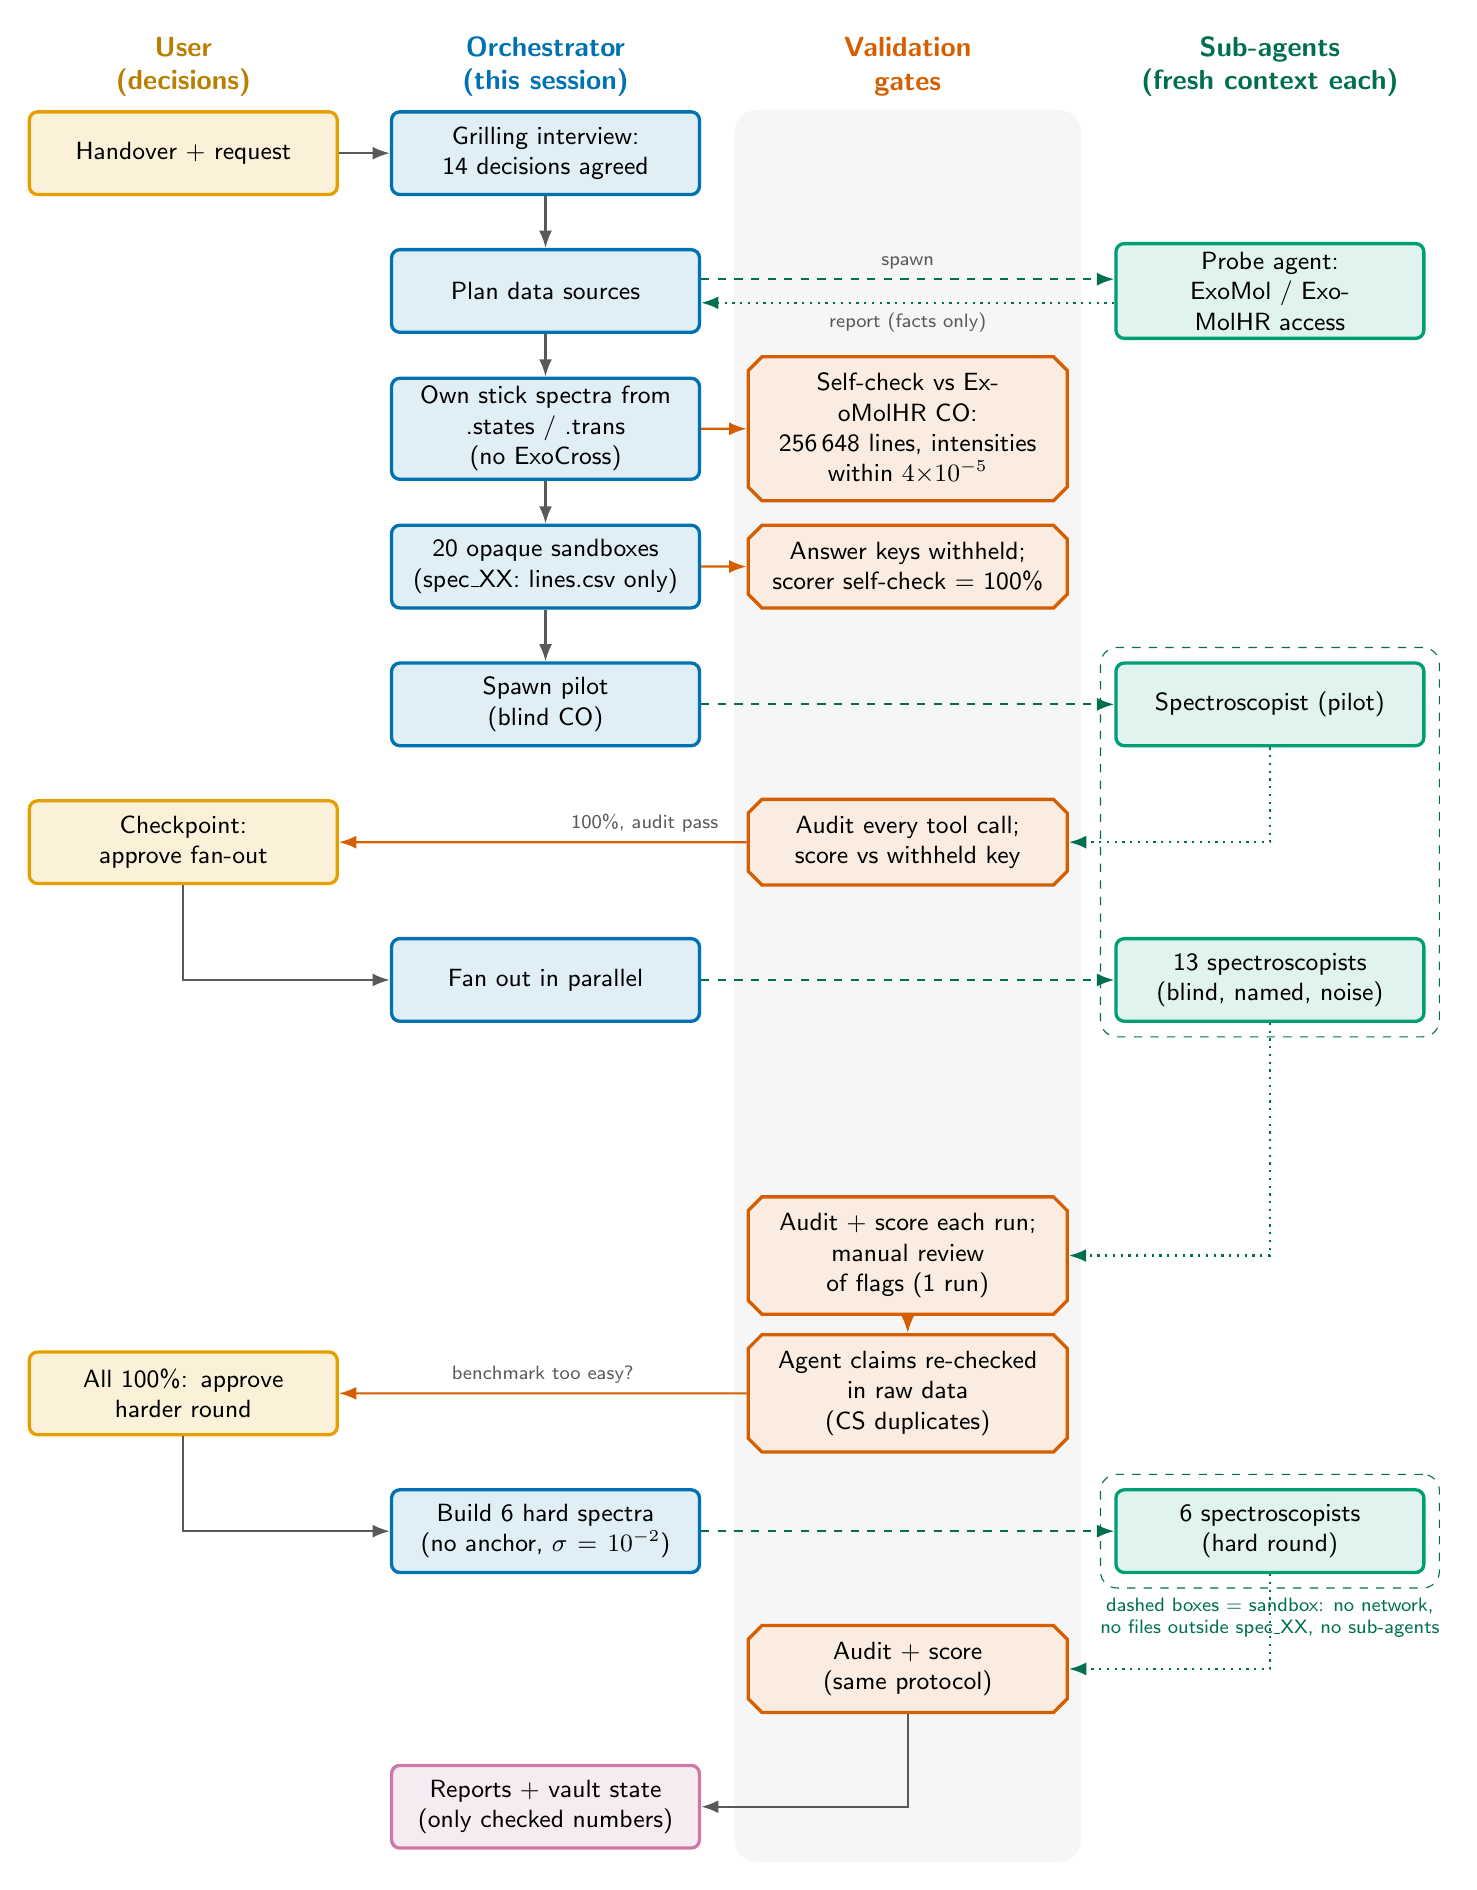
\begin{tikzpicture}[
    font=\sffamily\small,
    box/.style={rectangle, rounded corners=3pt, draw, very thick, align=center,
                text width=3.7cm, minimum height=1.05cm, inner sep=3pt},
    user/.style={box, draw=oiOrange, fill=oiOrange!15},
    orch/.style={box, draw=oiBlue, fill=oiBlue!12},
    agent/.style={box, draw=oiGreen, fill=oiGreen!12},
    gate/.style={box, draw=oiVermillion, fill=oiVermillion!12, chamfered rectangle,
                 chamfered rectangle xsep=2pt, rounded corners=0pt},
    outbox/.style={box, draw=oiPurple, fill=oiPurple!15},
    flow/.style={-{Latex[length=2.2mm]}, thick, arrowGrey},
    spawn/.style={-{Latex[length=2.2mm]}, thick, dashed, oiGreen!70!black},
    back/.style={-{Latex[length=2.2mm]}, thick, dotted, oiGreen!70!black},
    check/.style={-{Latex[length=2.2mm]}, thick, oiVermillion},
    lanehead/.style={font=\sffamily\bfseries, align=center},
    note/.style={font=\sffamily\scriptsize, align=center, text=arrowGrey},
    sandbox/.style={draw=oiGreen!70!black, dashed, rounded corners=6pt, inner sep=5pt},
]

% column x positions and row step
\def\xU{0}\def\xO{4.6}\def\xG{9.2}\def\xA{13.8}\def\dy{1.75}

% --- lane headings ---
\node[lanehead, text=oiOrange!80!black] at (\xU, 1.1) {User\\(decisions)};
\node[lanehead, text=oiBlue] at (\xO, 1.1) {Orchestrator\\(this session)};
\node[lanehead, text=oiVermillion] at (\xG, 1.1) {Validation\\gates};
\node[lanehead, text=oiGreen!70!black] at (\xA, 1.1) {Sub-agents\\(fresh context each)};

% --- row 1: scope ---
\node[user] (u1) at (\xU, 0) {Handover + request};
\node[orch] (o1) at (\xO, 0) {Grilling interview:\\14 decisions agreed};
\draw[flow] (u1) -- (o1);

% --- row 2: data access ---
\node[orch] (o2) at (\xO, -\dy) {Plan data sources};
\node[agent] (a2) at (\xA, -\dy) {Probe agent:\\ExoMol / ExoMolHR access};
\draw[flow] (o1) -- (o2);
\draw[spawn] (o2.east) ++(0,0.15) -- ($(a2.west)+(0,0.15)$) node[midway, above, note] {spawn};
\draw[back] ($(a2.west)+(0,-0.15)$) -- ($(o2.east)+(0,-0.15)$) node[midway, below, note] {report (facts only)};

% --- row 3: spectra ---
\node[orch] (o3) at (\xO, -2*\dy) {Own stick spectra from\\.states / .trans (no ExoCross)};
\node[gate] (g3) at (\xG, -2*\dy) {Self-check vs ExoMolHR CO:\\256\,648 lines, intensities\\within $4{\times}10^{-5}$};
\draw[flow] (o2) -- (o3);
\draw[check] (o3) -- (g3);

% --- row 4: sandboxes ---
\node[orch] (o4) at (\xO, -3*\dy) {20 opaque sandboxes\\(spec\_XX: lines.csv only)};
\node[gate] (g4) at (\xG, -3*\dy) {Answer keys withheld;\\scorer self-check = 100\%};
\draw[flow] (o3) -- (o4);
\draw[check] (o4) -- (g4);

% --- row 5: pilot ---
\node[orch] (o5) at (\xO, -4*\dy) {Spawn pilot\\(blind CO)};
\node[agent] (a5) at (\xA, -4*\dy) {Spectroscopist (pilot)};
\draw[flow] (o4) -- (o5);
\draw[spawn] (o5) -- (a5);

% --- row 6: pilot check + checkpoint ---
\node[gate] (g6) at (\xG, -5*\dy) {Audit every tool call;\\score vs withheld key};
\node[user] (u6) at (\xU, -5*\dy) {Checkpoint:\\approve fan-out};
\draw[back] (a5) |- (g6);
\draw[check] (g6) -- (u6) node[pos=0.25, above, note] {100\%, audit pass};

% --- row 7: fan-out ---
\node[orch] (o7) at (\xO, -6*\dy) {Fan out in parallel};
\node[agent] (a7) at (\xA, -6*\dy) {13 spectroscopists\\(blind, named, noise)};
\draw[flow] (u6) |- (o7);
\draw[spawn] (o7) -- (a7);

% --- row 8: per-run checks ---
\node[gate] (g8) at (\xG, -8*\dy) {Audit + score each run;\\manual review of flags (1 run)};
\node[gate] (g8b) at (\xG, -9*\dy) {Agent claims re-checked\\in raw data (CS duplicates)};
\draw[back] (a7.south) |- (g8.east);
\draw[check] (g8) -- (g8b);

% --- row 9: hard round ---
\node[user] (u9) at (\xU, -9*\dy) {All 100\%: approve\\harder round};
\node[orch] (o9) at (\xO, -10*\dy) {Build 6 hard spectra\\(no anchor, $\sigma=10^{-2}$)};
\node[agent] (a9) at (\xA, -10*\dy) {6 spectroscopists\\(hard round)};
\node[gate] (g9) at (\xG, -11*\dy) {Audit + score\\(same protocol)};
\draw[check] (g8b) -- (u9) node[midway, above, note] {benchmark too easy?};
\draw[flow] (u9) |- (o9);
\draw[spawn] (o9) -- (a9);
\draw[back] (a9) |- (g9);

% --- row 10: outputs ---
\node[outbox] (o10) at (\xO, -12*\dy) {Reports + vault state\\(only checked numbers)};
\draw[flow] (g9) |- (o10);

% --- sandbox boundary around spectroscopist agents ---
\begin{scope}[on background layer]
  \node[sandbox, fit=(a5)(a7)] {};
  \node[sandbox, fit=(a9), label={[note, text=oiGreen!70!black, align=center]below:dashed boxes = sandbox: no network,\\no files outside spec\_XX, no sub-agents}] {};
  \fill[laneBg, rounded corners=8pt] ($(\xG-2.2, 0.55)$) rectangle ($(\xG+2.2, -12*\dy-0.7)$);
\end{scope}

\end{tikzpicture}
\end{document}
